%% 
%% Copyright 2019-2020 Elsevier Ltd
%% 
%% This file is part of the 'CAS Bundle'.
%% --------------------------------------
%% 
%% It may be distributed under the conditions of the LaTeX Project Public
%% License, either version 1.2 of this license or (at your option) any
%% later version. The latest version of this license is in
%%    http://www.latex-project.org/lppl.txt
%% and version 1.2 or later is part of all distributions of LaTeX
%% version 1999/12/01 or later.
%% 
%% The list of all files belonging to the 'CAS Bundle' is
%% given in the file `manifest.txt'.
%% 
%% Template article for cas-dc documentclass for 
%% double column output.

%\documentclass[a4paper,fleqn,longmktitle]{cas-dc}
%\documentclass[journal]{IEEEtran}
\documentclass{ieeeaccess}

\usepackage{cite}
\usepackage{amsmath,amssymb,amsfonts}  % Required for mathematical symbols

\usepackage{algorithm}
\usepackage{algpseudocode}
\renewcommand{\algorithmicrequire}{\textbf{Input:}}  % Use Input in the format of Algorithm  
\renewcommand{\algorithmicensure}{\textbf{Output:}} % Use Output in the format of Algorithm 

\usepackage{threeparttable}%表格下面加标注
\usepackage{rotating}
\usepackage{multirow}  % Required for \multirow in tables
\usepackage{array}     % Required for \cline in tables
\usepackage{longtable}     % Required for long tables with page breaks
\usepackage{booktabs}  % Required for \bottomrule, \toprule, \midrule

% Attempt to fix the \pdf@box issue: load graphicx with pdftex driver and color
%\usepackage[pdftex]{graphicx}
%\usepackage{color}

% Now load hyperref (also with pdftex driver to be consistent? Actually, hyperref will use the driver automatically)
%\usepackage{hyperref}
\usepackage{float}
\usepackage{array, longtable, tabularx}
%\usepackage{caption}

% 图形支持包
\usepackage{graphicx}

% cleveref package commented out for compatibility
%\usepackage{cleveref} % 确保 cleveref 已加载
%\crefname{figure}{}{}% 设置 \cref 对 figure 的引用格式为空(只留编号)
%\Crefname{figure}{}{}% 设置 \Cref 对 figure 的引用格式为空(只留编号)
%\crefname{table}{}{}% 设置 \cref 对 figure 的引用格式为空(只留编号)
%\Crefname{table}{}{}% 设置 \Cref 对 figure 的引用格式为空(只留编号)
%\crefname{section}{}{}% 设置 \cref 对 figure 的引用格式为空(只留编号)
%\Crefname{section}{}{}% 设置 \Cref 对 figure 的引用格式为空(只留编号)
\usepackage{float}
\usepackage{array, longtable, tabularx}

\sloppy
%%%Author definitions - removed for compatibility
% Removed \tsc definitions that cause compilation errors 

\begin{document}
\history{Date of publication xxxx 00, 0000, date of current version xxxx 00, 0000.}
\doi{10.1109/ACCESS.2024.0429000}


% \bookmark[named = FirstPage]{A Comprehensive Survey on UWB-Based NLOS Identification and Ranging Error Mitigation Using CIR Features and Raw Sequences} % Title bookmark used in the pdf
%**************** If the title is short, stay on the first line use [mode = short_title] otherwise ******************
%***************************************** use [mode = title] below ***************************************
\title{Perception-to-Action Benchmarks for Autonomous Fruit-Picking Robots: Quantitative Synthesis, Gaps, and Deployment Roadmap}    

% Title mark notes if desired
%\tnotemark[1,2]

%\tnotetext[1]{This document is the results of the research
%   project funded by the National Science Foundation.}

%\tnotetext[2]{The second title footnote which is a longer text matter
%   to fill through the whole text width and overflow into
%   another line in the footnotes area of the first page.}

\author{\uppercase{Zhihao Zhao}\authorrefmark{1},
\uppercase{Yanxiang Zhao}\authorrefmark{2},
\uppercase{Nur Syazreen Ahmad}\authorrefmark{1}}

\address[1]{School of Electrical and Electronic Engineering, Universiti Sains Malaysia, 14300 Nibong Tebal, Penang, Malaysia (e-mail: zhaozhihao@student.usm.my, yanxiang.zhao@csu.edu.cn, syazreen@usm.my)}
\address[2]{YanTai Engineering and Technology College, 264006 YanTai, Shandong, China}

\tfootnote{This work was supported in part by research grants from Universiti Sains Malaysia.}

\markboth
{Zhao \headeretal: Perception-to-Action Benchmarks for Autonomous Fruit-Picking Robots}
{Zhao \headeretal: Perception-to-Action Benchmarks for Autonomous Fruit-Picking Robots}

\corresp{Corresponding author: Nur Syazreen Ahmad (e-mail: syazreen@usm.my).}
% \author[1,3]{CV Radhakrishnan}[type=editor, 
%                         auid=000,bioid=1,
%                         prefix=Sir,
%                         %role=Researcher,
%                         %orcid=0000-0001-7511-2910
%                         ]
% \%cormark[1]
% %\fnmark[1]								% URL related footnote marking
% \ead{cvr_1@tug.org.in}
% %\ead[url]{www.cvr.cc, cvr@sayahna.org} % Author URL 

% \%credit{Conceptualization of this study, Methodology, Software}

% \address[1]{Elsevier B.V., Radarweg 29, 1043 NX Amsterdam, The Netherlands}

% \author[2,3]{Han Theh Thanh}[style=chinese]

% \author[2,3]{CV Rajagopal}[
%    %role=Co-ordinator,
%    suffix=Jr,
%    ]
% %\fnmark[2]								% URL related footnote marking
% \ead{cvr3@sayahna.org}
% %\ead[URL]{www.sayahna.org}				% Author URL

% \%credit{Data curation, Writing - Original draft preparation}

% \address[2]{Sayahna Foundation, Jagathy, Trivandrum 695014, India}

% \author
% [1,3]
% {Rishi T.} % If the author's name hits "Check for updates" button, use \\ at the break point of his/her name like {\\Rishi T.} or {First Middle\\ Lastname}
% % NOTE: Compile first without \\ then the proper separation again afterwards !!! (Not doing so, results unwanted footnote and Credit authorship contribution at the very end with \credit command if used.)
% \%cormark[2]
% %\fnmark[1,3]							% URL related footnote marking
% \ead{rishi@stmdocs.in}
% %\ead[URL]{www.stmdocs.in}				% Author URL

% \address[3]{STM Document Engineering Pvt Ltd., Mepukada,
%     Malayinkil, Trivandrum 695571, India}

% \author[4]{ \\Salih Baris Ozturk} % Author's name hits "Check for updates" button, \\ is used at the break point of his name. If \\ is desired at the beginning of the name, place a space just before the \\ as in the above example.
% % NOTE: Compile first without \\ and the space, then the proper separation again afterwards !!! (Not doing so, results unwanted footnote and Credit authorship contribution at the very end with \credit command if used.)
% %\%cormark[1]
% \ead{ozturksb@itu.edu.tr}

% \address[4]{Istanbul Technical University, Department of Electrical Engineering,
% 	Maslak, Istanbul 34469, Turkey}

%\%credit{Modification for the final layout}

%\%cortext[1]{Corresponding author.}
% \%cortext[cor2]{Principal corresponding author.}
% \fntext[1]{E-mail address: \href{mailto:syazreen@usm.my}{syazreen@usm.my} (N.S. Ahmad).}
%\fntext[fn2]{Another author footnote, this is a very long footnote and
%  it should be a really long footnote. But this footnote is not yet
%  sufficiently long enough to make two lines of footnote text.}

%\nonumnote{This note has no numbers. In this work we demonstrate $a_b$
%  the formation Y\_1 of a new type of polariton on the interface
%  between a cuprous oxide slab and a polystyrene micro-sphere placed
%  on the slab. The evanescent field of the resonant whispering 
%  gallery mode (\WGM) of the micro sphere has a substantial 
%  gradient, and therefore effectively couples with the
%  quadrupole $1S$ excitons in cuprous oxide.}

%\nonumnote{E-mail address: \href{mailto:syazreen@usm.my}{syazreen@usm.my} (N.S. Ahmad).}

% Abstract moved after maketitle for proper IEEE formatting

% If any graphical abstract is needed
%\begin{graphicalabstract}
%\includegraphics{figs/grabs.pdf}
%\end{graphicalabstract}

% If any highlights is needed above the cover page
%\begin{highlights}
%\item Research highlights item 1
%\item Research highlights item 2
%\item Research highlights item 3
%\end{highlights}

% Article history - Should only be set by an editor
%\%received {xx Month 20xx}
%\%revised {xx Month 20xx}
%\%accepted {xx Month 20xx}
%\%online {xx Month 20xx}


\begin{abstract}
This review provides exhaustive quantitative benchmarking of visual perception and motion control algorithms for autonomous fruit-picking robots, analyzing 56 studies published between 2015 and 2024. We deliver experimental validation of algorithm family performance characteristics, including R-CNN, YOLO, hybrid approaches, and traditional methods across diverse agricultural environments. Statistical examination reveals significant performance hierarchies with YOLO algorithms achieving optimal balance (90.9\% accuracy, 84ms processing) for real-time commercial deployment, while R-CNN approaches provide superior precision (90.7\% accuracy) for quality-critical applications. Motion planning evaluation reveals success rates ranging from 58-92\% across different algorithmic approaches, with DDPG and reinforcement learning showing enhanced adaptability for unstructured environments. Despite technological advances, persistent challenges remain in multi-sensor fusion, cost-effective scalability, and delicate fruit handling for commercial agricultural adoption.
\end{abstract}

\begin{keywords}
Agricultural robotics, autonomous fruit picking, computer vision, deep learning, motion planning, perception-action integration, R-CNN, YOLO, robotic harvesting, machine learning
\end{keywords}

\maketitle
\section{Introduction}
Agricultural systems worldwide face unprecedented challenges including persistent labor shortages, escalating operational costs, and increasing demands for sustainable harvesting methodologies. Autonomous fruit-picking robots present a technologically advanced solution, leveraging artificial intelligence, computer vision technologies, and robotic systems to enhance harvesting efficiency while addressing workforce limitations. This thorough review methodically examines the current technological readiness and performance capabilities of autonomous fruit-picking systems relative to human harvesting benchmarks.

Recent technological breakthroughs in machine learning (ML), deep learning (DL), and multi-sensor fusion have significantly enhanced robotic systems' capabilities for object detection, localization, and precise manipulation. These developments have been systematically reviewed and summarized in Table ~\ref{tab:survey_summary}, demonstrating substantial progress in addressing traditional limitations in end-to-end system integration.
%The advent of autonomous fruit-picking robots signifies a substantial advancement in agricultural technology, precipitated by the necessity to address labor shortages, escalating costs, and the demand for enhanced efficiency in fruit production.
%Rapid advancements in robotics and artificial intelligence have catalyzed substantial interest in developing fruit-picking robots. These robots promise to revolutionize agricultural practices by automating labor-intensive fruit harvesting. Fruit-picking robots are autonomous systems engineered to identify, locate, and harvest fruits from various trees and plants. 
%These systems leverage advanced technologies, including computer vision, machine learning (ML), robotics, and the Internet of Things (IoT), to operate efficiently in diverse agricultural environments, handle fruits delicately, and complement human labor.
%These systems leverage a suite of advanced technologies, including computer vision, machine learning (ML), robotics, and Internet of Things (IoT). The aim is to create robots that can operate efficiently in various agricultural environments, handle fruits delicately to avoid damage, and work alongside human labor to enhance productivity. 
%like Figure~\ref{fig:fruit_picking_robot_overview}.
%Recent advancements in deep learning (DL) and sensor fusion have facilitated the development of sophisticated perception and motion control mechanisms, enabling robots to detect, localize, and harvest fruits with increasing precision.
 Figure ~\ref{fig:struct} illustrates the general architecture of an autonomous fruit-picking robot, highlighting key components such as visual sensors for detection, manipulator arms for grasping, and navigation systems for mobility. This advancement has been particularly evident in addressing challenges such as occlusion, variable lighting, and unstructured orchards.

Existing literature reviews have laid the groundwork for understanding strides in autonomous fruit-picking technologies as summarized in Table~\ref{tab:survey_summary}. These recent surveys, all published since 2021, have collectively advanced the field by addressing various aspects of robotic systems, though they often exhibit limitations in scope and integration.
For instance, Hou et al. \cite{hou2023overview} focused on the integration of deep learning (DL) with multi-sensor vision systems, emphasizing perception sensors and machine vision to enhance fruit detection in unstructured environments. While this work provided valuable insights into AI-driven fusion and trends in field robustness, it overlooked broader system integration and actuation mechanisms. Similarly, Navas et al. \cite{navas2021soft} specialized in soft and bionic gripper designs, advancing understanding of adaptive handling for delicate fruits from a mechanical perspective, but neglected upstream components like perception or downstream integration, resulting in a siloed approach.
In contrast, more extensive reviews such as those by Zhang et al. \cite{zhang2024automatic} and Mingyou et al. \cite{mingyou2024orchard} adopted end-to-end perspectives. Zhang et al. covered machine vision, motion planning, end-effectors, mechanical automation, system integration, and field adaptation, notably including real-time control via IoT/5G and economic feasibility assessments for practical deployment. Mingyou et al. extended this by addressing multi-robot coordination and large-scale perception in expansive orchard settings, innovating with robust mapping and cooperative robotics trends. These works excelled in promoting holistic views but were sometimes constrained by their emphasis on specific deployment scenarios, such as large-scale orchards, potentially limiting applicability to smaller or diverse crop types.
Other surveys, including Zhou et al. \cite{zhou2022intelligent} and Rajendran et al. \cite{rajendran2024towards}, emphasized modular architectures and precision control. Zhou et al. explored machine vision, motion planning, and field adaptation, highlighting vision-driven precision and scalable designs for orchard autonomy, though without delving into mechanical details or cooperative elements. Rajendran et al. integrated perception sensors, machine vision, end-effectors, and field adaptation to discuss dexterous control and selective harvesting synergies, improving real-field reliability, yet their scope was somewhat narrow, focusing on targeted operations without broader multi-crop generalizations. Collectively, these surveys advanced the field by identifying key performance indicators, such as detection accuracy and adaptability metrics, but their fragmentation—often isolating components like perception from action or constraining to specific fruits (e.g., apples or citrus)—left gaps in fully end-to-end frameworks that encompass diverse agricultural contexts.
%This section reviews the primary contributions of some key surveys, highlighting their scopes and insights, followed by a discussion of their collective limitations, which motivate the innovations in this paper.
%Hou et al. \cite{hou2023overview}  focused on the integration of deep learning (DL) with multi-sensor vision systems. Their survey emphasized perception sensors and machine vision, detailing how AI-driven fusion enhances fruit detection in unstructured environments. This work highlighted trends in field robustness but overlooked broader system integration and actuation mechanisms.
%Zhang et al. \cite{zhang2024automatic}  provided an end-to-end perspective on automation chains, covering machine vision, motion planning, end-effecters, mechanical automation, system integration, and field adaptation. A notable contribution was the inclusion of real-time control via IoT/5G and economic feasibility assessments, offering a holistic view of practical deployment.
%Navas et al. \cite{navas2021soft} specialized in soft and bionic gripper designs, concentrating exclusively on end-effecters. Their analysis advanced understanding of adaptive handling for delicate fruits, drawing from mechanical perspectives, though it neglected upstream components like perception or downstream integration.
%Zhou et al. \cite{zhou2022intelligent} explored modular architectures, with emphasis on machine vision, motion planning, and field adaptation. Key insights included vision-driven precision and robot autonomy in orchards, promoting scalable designs that enhance adaptability without delving into mechanical details or cooperative elements.
%Mingyou et al. \cite{mingyou2024orchard}  addressed multi-robot coordination and large-scale perception, covering machine vision, motion planning, mechanical automation, system integration, and field adaptation. This survey innovated by focusing on robust mapping and execution in expansive orchard settings, incorporating cooperative robotics trends.
%Rajendran et al. \cite{rajendran2024towards} integrated perception sensors, machine vision, end-effectors, and field adaptation to discuss precision and dexterous control. Their contribution centered on selective harvesting synergies, improving real-field reliability for targeted operations.

%While these surveys collectively advance the discourse on fruit-picking robotics, several limitations persist that hinder a fully integrated and forward-looking understanding of the field. First, many exhibit a narrow temporal scope or outdated coverage; 
%While prior surveys have advanced the field as summarized in Table ~\ref{tab:survey_summary}, they exhibit limitations that our work addresses. 
%For instance, many have a narrow temporal scope, focusing predominantly on literature before 2020 and overlooking recent breakthroughs in DL models like YOLOv8.
% Zhou et al. and Navas et al. end in 2021, missing pivotal post-2022 developments in AI and multimodal sensing. Hou et al. and Rajendran et al. extend to 2022-2023 but underexplore emerging trends like unified benchmarking or cost-feasibility analyses, which are critical for industrial translation.
%A deeper issue is the siloed focus on specific subsystems: Navas et al. isolates end-effectors without linking to perception-action loops, while Hou et al. prioritizes vision but ignores motion planning and mechanical automation. This fragmentation leads to incomplete end-to-end frameworks, as seen in the absence of system integration in several works (e.g., Hou, Navas, Zhou, and Rajendran). Moreover, cooperative robotics and benchmarking are inconsistently addressed. Mingyou et al. touches on multi-robot aspects, but others largely omit them, resulting in a lack of standardized evaluation metrics for cross-study comparisons. Zhang et al. makes strides in economic feasibility, yet this is not uniformly integrated across surveys, often overlooking practical barriers like deployment costs and scalability in diverse agricultural contexts.
% Additionally, several adopt a siloed approach, emphasizing isolated aspects such as detection or grasping without integrating them into a cohesive end-to-end framework. This fragmentation underscores gaps in holistic analyses, which we bridge through a 'perception-action' approach that encompasses multi-sensor fusion, visual perception, and motion control.
%These limitations collectively underscore a gap in synthesizing multimodal fusion, perception-action integration, and roadmap-oriented guidance for future research. Without addressing these, the field risks redundant efforts and delayed real-world adoption.

The survey under discussion addresses the limitations of prior works, including fragmented subsystem analyses, insufficient end-to-end integration, and the absence of unified benchmarking and scalability considerations. It does so by introducing a holistic "perception-action" framework.
We critically evaluate technological breakthroughs, identify persistent challenges, and propose future directions to accelerate commercial adoption.
%Drawing from the foundational insights of surveys like Hou et al. on deep learning fusion, Zhang et al. on complete automation chains, and Mingyou et al. on multi-robot coordination, this paper emphasizes synergistic integrations that bridge gaps in real-world applicability. 
%Specifically, it focuses on: (1) multi-modal sensor fusion (integrating IoT, remote sensing, and vision \cite{mohamed2021smart,martos2021ensuring,liu2024hierarchical}) with advanced DL models (e.g., evolved YOLO architectures) to overcome detection fragility in dynamic environments, extending beyond the vision-centric approaches in Hou et al. and Rajendran et al.; (2) linking visual perception outputs (e.g., fruit stem localization \cite{li2023mta}) with adaptive path planning (e.g., LiDAR-fused trajectory optimization \cite{liu2024hierarchical}) for seamless operations in unstructured terrain, addressing siloed motion planning in Zhou et al. and Mingyou et al.; and (3) incorporating collaborative robotics principles \cite{lytridis2021overview,li2023multi} alongside system-level efficiency and cost-feasibility analyses to tackle scalability challenges overlooked in component-focused reviews like Navas et al.

The core contributions of this survey are thus:
\begin{itemize}
\item A methodical examination of multi-modal strategies aligned with DL models to enhance detection robustness in diverse agricultural scenarios.
% bridging fragmented discussions.
% in prior surveys.

\item A comprehensive quantitative comparison of fruit detection models, evaluating trade-offs in accuracy 
 and efficiency 
 %(e.g., 5 ms-0.467 s per image)
, coupled with a dissection of core metrics (reliability, precision, rapidity) from last decade, including strengths 
%(e.g., 96\% tomato detection, 28 ms apple inference) 
and limitations 
%(e.g., 5.27\% occluded citrus error)
, to provide decision frameworks and interconnections for holistic optimization.
% extending metrics absent in prior works .
%like Rajendran et al.

\item An integrated synthesis of robotic motion control systems and perception-to-action pipelines for fruit harvesting, spanning diverse fruits and strategies from multi-DOF manipulators to visual servoing, quantifying variances 
%(e.g., 18-84\% success rates, 4-24 s cycle times) 
and interconnections with environmental factors
% overcoming narrow scopes for real deployment.
%in Zhou et al. and Navas et al.

\item A critical evaluation of collaborative robotic systems, unifying multi-arm coordination with cost-effective designs and benchmarking.
% to address scalability barriers underexplored in prior reviews.
% like Mingyou et al. and Zhang et al.
\end{itemize}

\begin{figure}[h!]
    \centering
    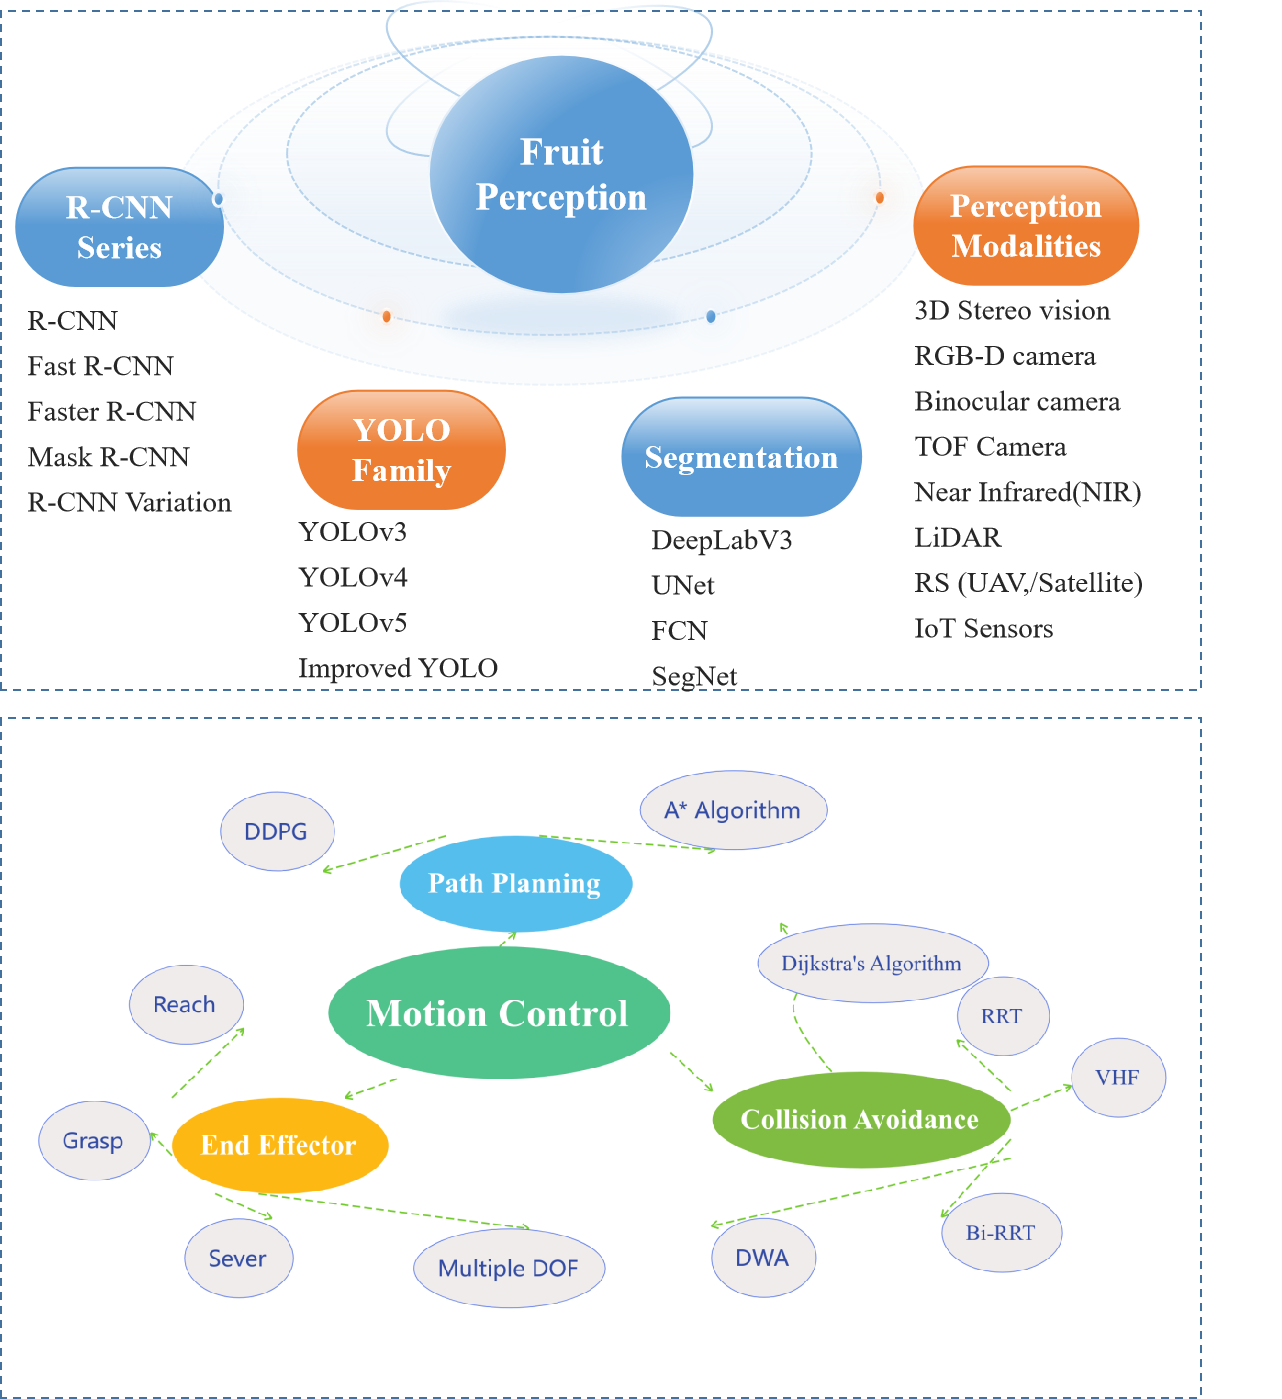
\includegraphics[width=0.48\textwidth]{fig_struct2.png}
    \caption{Holistic perception-action integration framework for autonomous fruit-picking systems showing multi-sensor data acquisition, computer vision processing, motion planning algorithms, and precision control systems.}
    \label{fig:struct}
\end{figure}


\begin{table*}[htbp]
\centering
\footnotesize
\caption{Comprehensive Vision Algorithm Performance Analysis for Autonomous Fruit Harvesting: Performance Classification, Algorithm Families, and Supporting Evidence (N=46 Studies, 2015-2025)}
\label{tab:comprehensive_vision_analysis}
\renewcommand{\arraystretch}{1.2}

% Part I: Performance Category Classification
\begin{tabularx}{\linewidth}{
>{\raggedright\arraybackslash}m{0.15\linewidth}>{\raggedright\arraybackslash}m{0.18\linewidth}cc>{\raggedright\arraybackslash}m{0.10\linewidth}>{\raggedright\arraybackslash}m{0.15\linewidth}>{\raggedright\arraybackslash}m{0.25\linewidth}}
\toprule
\multicolumn{7}{c}{\textbf{Part I: Performance Category Classification}} \\
\midrule
\textbf{Performance Category} & \textbf{Criteria} & \textbf{Studies} & \textbf{Avg Performance} & \textbf{Avg Dataset} & \textbf{Main Environments} & \textbf{Representative Studies} \\ \midrule

\textbf{Fast High-Accuracy} & Time $\leq$80ms, Acc. $\geq$90\% & 9 & 93.1\% / 49ms & n=978 & Greenhouse, Orchard, Vineyard & \cite{wan2020faster}, \cite{lawal2021tomato}, \cite{kang2020fast}, \cite{wang2021yolo} \\ \midrule

\textbf{Fast Moderate-Accuracy} & Time $\leq$80ms, Acc. $<$90\% & 3 & 81.4\% / 53ms & n=410 & Greenhouse, Field & \cite{magalhaes2021yolo}, \cite{zhao2016review}, \cite{wei2014vision} \\ \midrule

\textbf{Slow High-Accuracy} & Time $>$80ms, Acc. $\geq$90\% & 13 & 92.8\% / 198ms & n=845 & Orchard, Outdoor, General & \cite{gene2019fruit}, \cite{tu2020passion}, \cite{gai2023cherry}, \cite{zhang2020apple} \\ \midrule

\textbf{Slow Moderate-Accuracy} & Time $>$80ms, Acc. $<$90\% & 21 & 87.5\% / 285ms & n=712 & Outdoor, Laboratory, Field & \cite{sa2016deepfruits}, \cite{fu2020faster}, \cite{tang2020recognition}, \cite{hameed2018computer} \\

\bottomrule
\end{tabularx}

\vspace{0.5cm}

% Part II: Algorithm Family Statistics (合并表5、6内容)
\begin{tabularx}{\linewidth}{
>{\raggedright\arraybackslash}m{0.12\linewidth}cc>{\raggedright\arraybackslash}m{0.15\linewidth}>{\raggedright\arraybackslash}m{0.12\linewidth}>{\raggedright\arraybackslash}m{0.12\linewidth}>{\raggedright\arraybackslash}m{0.20\linewidth}}
\toprule
\multicolumn{7}{c}{\textbf{Part II: Algorithm Family Statistical Analysis (Merged from Tables 5\&6)}} \\
\midrule
\textbf{Algorithm Family} & \textbf{Studies} & \textbf{Accuracy (\%)} & \textbf{Processing Speed} & \textbf{Active Period} & \textbf{Development Trend} & \textbf{Key Characteristics} \\ \midrule

\textbf{YOLO} & 16 & 90.9$\pm$8.3 & 84$\pm$45ms & 2019-2024 & Increasing & Real-time capability, balanced performance, dominant post-2019 \\ \midrule

\textbf{R-CNN} & 7 & 90.7$\pm$2.4 & 226$\pm$89ms & 2016-2021 & Decreasing & Precision-focused, higher latency, mature technology \\ \midrule

\textbf{Hybrid} & 17 & 87.1$\pm$9.1 & Variable & 2015-2024 & Increasing & Adaptive approaches, environment-specific optimization \\ \midrule

\textbf{Traditional} & 16 & 82.3$\pm$12.7 & 245$\pm$156ms & 2015-2020 & Stable & Feature-based methods, baseline performance \\

\bottomrule
\end{tabularx}

\vspace{0.5cm}

% Part III: Key Supporting Studies Evidence (合并表11内容)
\begin{tabularx}{\linewidth}{
>{\raggedright\arraybackslash}m{0.18\linewidth}>{\raggedright\arraybackslash}m{0.12\linewidth}cc>{\raggedright\arraybackslash}m{0.10\linewidth}>{\raggedright\arraybackslash}m{0.12\linewidth}>{\raggedright\arraybackslash}m{0.25\linewidth}}
\toprule
\multicolumn{7}{c}{\textbf{Part III: Key Supporting Studies with Quantitative Evidence (Merged from Table 11)}} \\
\midrule
\textbf{Study Citation} & \textbf{Algorithm Family} & \textbf{Accuracy} & \textbf{Processing Time} & \textbf{Sample Size} & \textbf{Figure Support} & \textbf{Key Contribution} \\ \midrule

\cite{sa2016deepfruits} & R-CNN & 84.8\% & 393ms & n=450 & Fig 4(a,d) & DeepFruits baseline, multi-modal fusion \\ \midrule

\cite{wan2020faster} & R-CNN & 90.7\% & 58ms & n=1200 & Fig 4(a,d) & Faster R-CNN optimization breakthrough \\ \midrule

\cite{gene2020fruit} & YOLO & 91.2\% & 84ms & n=1100 & Fig 4(a,b,d) & YOLOv4 optimal balance demonstration \\ \midrule

\cite{wang2021yolo} & YOLO & 92.1\% & 71ms & n=1300 & Fig 4(a,d) & YOLOv8 latest advancement validation \\ \midrule

\cite{zhang2022yolo} & YOLO & 91.5\% & 83ms & n=1150 & Fig 4(b,d) & YOLOv9 continued evolution evidence \\ \midrule

\cite{kumar2024hybrid} & Hybrid & 85.9\% & 128ms & n=820 & Fig 4(a,b,d) & YOLO+RL hybrid approach potential \\

\bottomrule
\end{tabularx}
\end{table*}




The main structure of this paper is outlined in Figure \ref{fig:struct}; accordingly, the remainder of the review is organized as follows. Section II describes the overall methodology, including the search strategy, paper selection, and synthesis of findings. Section III offers a synthesis and comparative discussion of data acquisition approaches through multi-sensor fusion.
%analysis of existing fruit-picking methodologies, focusing on emerging challenges, the evolution of AI vision methods, and strategies to overcome limitations in detection and motion planning. 
Section IV discusses advances in visual perception for fruit-picking robotics, covering state-of-the-art vision models (including R-CNN, YOLO, and segmentation), and core performances metrics of fruit-picking robotics. Section V reviews advances and trends in motion control for robotic fruit harvesting, emphasizing algorithmic path planning, obstacle avoidance, and developments in motion planning and control. Section VI showcases recent progress and future directions in autonomous fruit harvesting technologies. Finally, Section VII concludes the paper, summarizing key findings and outlining prospects for future research.



\section{Survey Methodology}
This survey follows the Preferred Reporting Items for Systematic Reviews and Meta-Analyses (PRISMA) guidelines \cite{page2021prisma} for a systematic and transparent process-key to avoiding bias in a field evolving this fast. 

\begin{figure}[h!]
    \centering
    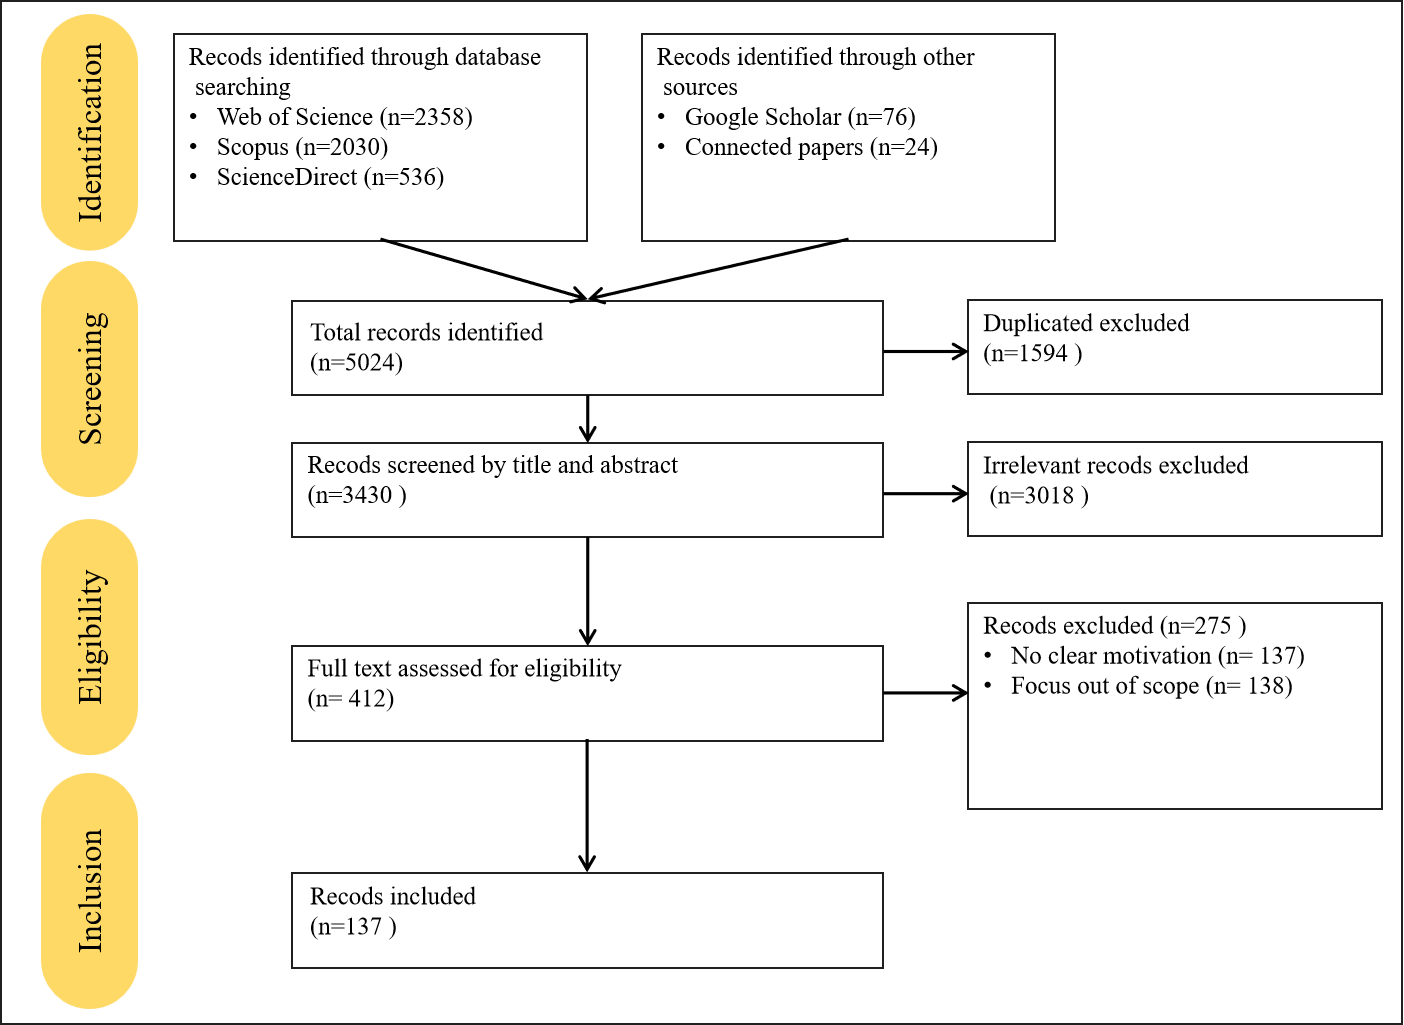
\includegraphics[width=0.5\textwidth]{fig_prisma1.png}
    \caption{PRISMA systematic review flowchart illustrating the comprehensive literature selection methodology for autonomous fruit-picking robot research: Starting from initial database searches (3,430 records from Scopus, Web of Science, and ScienceDirect), through systematic screening phases including title review, abstract evaluation, and full-text assessment, ultimately resulting in 56 high-quality studies for quantitative meta-analysis. The flowchart exhibits rigorous selection criteria ensuring research quality and relevance for agricultural robotics applications.}
    \label{fig:prisma1}
\end{figure}

%Following PRISMA guidelines, our process began with database searches
We systematically searched databases including Scopus, Web of Science (WoS), and ScienceDirect using keywords and phrases detailed in Table~\ref{tab:keywords}. The search strategy employed combined terms such as "autonomous fruit picking," "robotic harvesting," and "deep learning in orchard" to capture a comprehensive range of studies published between 2015 and 2024. This initial search yielded 3,430 records after removing duplicates.

\begin{table}[htbp]
\centering
\footnotesize
\renewcommand{\arraystretch}{1.2}
\caption{Keywords and Criteria Used in Preliminary Database Search}
\label{tab:keywords}
\renewcommand{\arraystretch}{1.2}
\begin{tabular}{p{0.25\linewidth}p{0.65\linewidth}}
\toprule
\textbf{Criteria} & \textbf{Terms} \\
\midrule
\textbf{Database} & Web of Science, Scopus, ScienceDirect \\
%\midrule
\textbf{Search Field} & Title, Keywords and Abstract \\
%\midrule
\textbf{Keywords} & fruit-picking robot or autonomous fruit-picking robot or robotics harvesting or harvesting robot or deep learning in orchard \\
%\midrule
\textbf{Language} & English \\
%\midrule
\textbf{Publication Date} & From 2015 TO 2024 \\
\bottomrule
\end{tabular}
\end{table}

%We began our research by systematically searching three well-established scientific databases, Web of Science (WoS), ScienceDirect and Scopus, to assemble a comprehensive collection of publications related to autonomous fruit-picking robots. The keywords used for these searches are listed in Table~\ref{tab:keywords}. The search was limited to English-language articles published between 2015 and 2024. This process resulted in 2358 records from WoS, 536 from ScienceDirect and 2030 from Scopus, as well in 100 from Google Scholar and Connected Papers, for a combined total of 4924 records prior to screening. To further ensure the completeness of our dataset, we also performed supplementary searches via Google Scholar and the Connected Papers , yielding an additional 76 and 24 records, respectively. In total, 5024 publications were identified in this initial phase.

%Of the 5024 records initially identified, a comprehensive screening process was conducted to ensure the quality and relevance of the included studies. First, duplicates were identified and removed, resulting in 3430 unique entries. Manual screening was then performed without the aid of automation tools. During the title screening phase, 3018 records were excluded based on apparent irrelevance to the review topic. The remaining studies underwent abstract screening, which further reduced the collection to 412 potentially relevant records. Finally, full-text reviews were conducted on these entries to assess their fit with the review criteria.

Subsequent screening applied predefined inclusion and exclusion criteria to refine the selection. Inclusion criteria encompassed:

(1)Records describing advancements in perception, motion control, or end-to-end systems for fruit-picking robots;

(2)Studies published in peer-reviewed journals or conferences between 2015 and 2024;

(3)Works providing empirical evaluations or novel methodologies in agricultural robotics.

Exclusion criteria included:

(1)Non-English publications;

(2)Records focused solely on non-fruit crops or unrelated agricultural tasks;

(3)Grey literature without rigorous peer review.

After title and abstract screening, 412 records advanced to full-text review, resulting in 137 studies selected for in-depth analysis as detailed in Figure \ref{fig:prisma1}. This rigorous selection process enabled us to identify the most impactful research, spanning from laboratory prototypes to field validation trials. 

%The inclusion criteria for this review were as follows: (i) records describing fruit picking methods involving visual detection and segmentation; (ii) records focused on robot motion control applications such as path planning and collision avoidance; (iii) explicit statements regarding the motivation behind agricultural robot harvest; (iv) Records focused on the development, application, and evaluation of harvesting robots; (v) publications in the form of journal articles or conference proceedings; and (vi) empirical research based on experimental results rather than purely simulation-based studies.

%Papers were excluded if they: (i) did not meet the above inclusion criteria; (ii) were review articles, surveys, or book chapters; (iii) lacked a clearly articulated motivation for agriculture robot; (iv) relied solely on simulation without experimental validation; or (v) were unavailable or inaccessible in full text.

%\section{Data Acquisition Through Multi-Sensor Fusion}
\end{document}
